\documentclass{article}
\usepackage{pgfplots}
\pgfplotsset{compat=1.17}
\usepackage{amsmath}
\usepackage{tikz}
\usetikzlibrary{plotmarks}

\begin{document}

%=======================
% Figura 1: Rastrigin
%=======================
\begin{center}
\begin{tikzpicture}
\begin{axis}[
    title={Rastrigin's Function},
    xlabel=$x$, ylabel=$y$, zlabel={$f(x,y)$},
    view={120}{25},
    domain=-5:5,
    domain y=-5:5,
    samples=100,
    samples y=100,
    colormap/hot,
]
\addplot3[surf] 
    {20 + x^2 + y^2 - 10*(cos(deg(2*pi*x)) + cos(deg(2*pi*y)))};
\end{axis}
\end{tikzpicture}
\end{center}

\vspace{2cm}

%=======================
% Figura 2: 3D scatterplot Iris
%=======================
\begin{center}
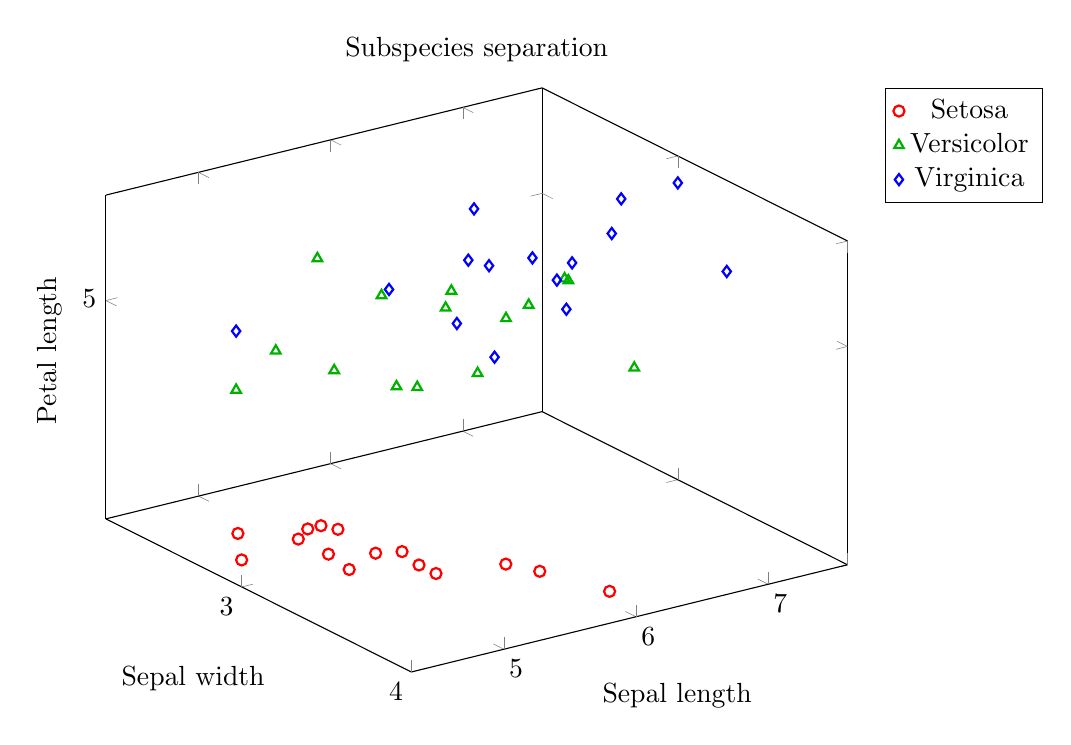
\begin{tikzpicture}
\begin{axis}[
    title={Subspecies separation},
    view={55}{30},
    xlabel={Sepal width},
    ylabel={Sepal length},
    zlabel={Petal length},
    xtick={4,3,2},
    ytick={4,5,6,7},
    ztick={5},
    legend style={at={(1.05,1)}, anchor=north west},
    width=11cm,
    height=9cm,
]

% Setosa – cercuri goale roșii
\addplot3[
    only marks,
    mark=o,
    mark options={draw=red, fill=none, thick},
]
table {
  3.5 5.0 1.4
  3.0 4.9 1.4
  3.2 4.7 1.3
  3.1 4.6 1.5
  3.6 5.0 1.4
  3.9 5.4 1.7
  3.4 4.6 1.4
  3.4 5.0 1.5
  2.9 4.4 1.4
  3.1 4.9 1.5
  3.7 5.4 1.5
  3.4 4.8 1.6
  3.0 4.8 1.4
  3.0 4.3 1.1
  4.0 5.8 1.2
};
\addlegendentry{Setosa}

% Versicolor – triunghiuri goale verzi
\addplot3[
    only marks,
    mark=triangle,
    mark options={draw=green!70!black, fill=none, thick},
]
table {
  2.8 7.0 4.7
  2.6 6.4 4.5
  2.9 6.9 4.9
  3.1 5.5 4.0
  3.6 6.5 4.6
  3.3 5.7 4.5
  3.0 6.3 4.7
  2.5 4.9 3.3
  2.9 6.6 4.6
  2.5 5.2 3.9
  3.0 5.0 4.5
  2.2 5.9 4.8
  2.5 6.0 4.5
  2.8 6.1 4.7
  2.9 5.6 3.6
};
\addlegendentry{Versicolor}

% Virginica – romburi goale albastre
\addplot3[
    only marks,
    mark=diamond,
    mark options={draw=blue, fill=none, thick},
]
table {
  3.3 6.3 6.0
  2.7 5.8 5.1
  3.0 7.1 5.9
  2.9 6.3 5.6
  3.0 6.5 5.8
  3.0 7.6 6.6
  2.5 4.9 4.5
  2.9 7.3 6.3
  2.5 6.7 5.8
  3.6 7.2 6.1
  3.2 6.5 5.1
  2.7 6.4 5.3
  3.0 6.8 5.5
  3.4 5.7 5.0
  3.1 5.8 5.1
};
\addlegendentry{Virginica}

\end{axis}
\end{tikzpicture}
\end{center}

\end{document}
